\section{Base\-Activity Class Reference}
\label{classBaseActivity}\index{BaseActivity@{BaseActivity}}
Inheritance diagram for Base\-Activity:\begin{figure}[H]
\begin{center}
\leavevmode
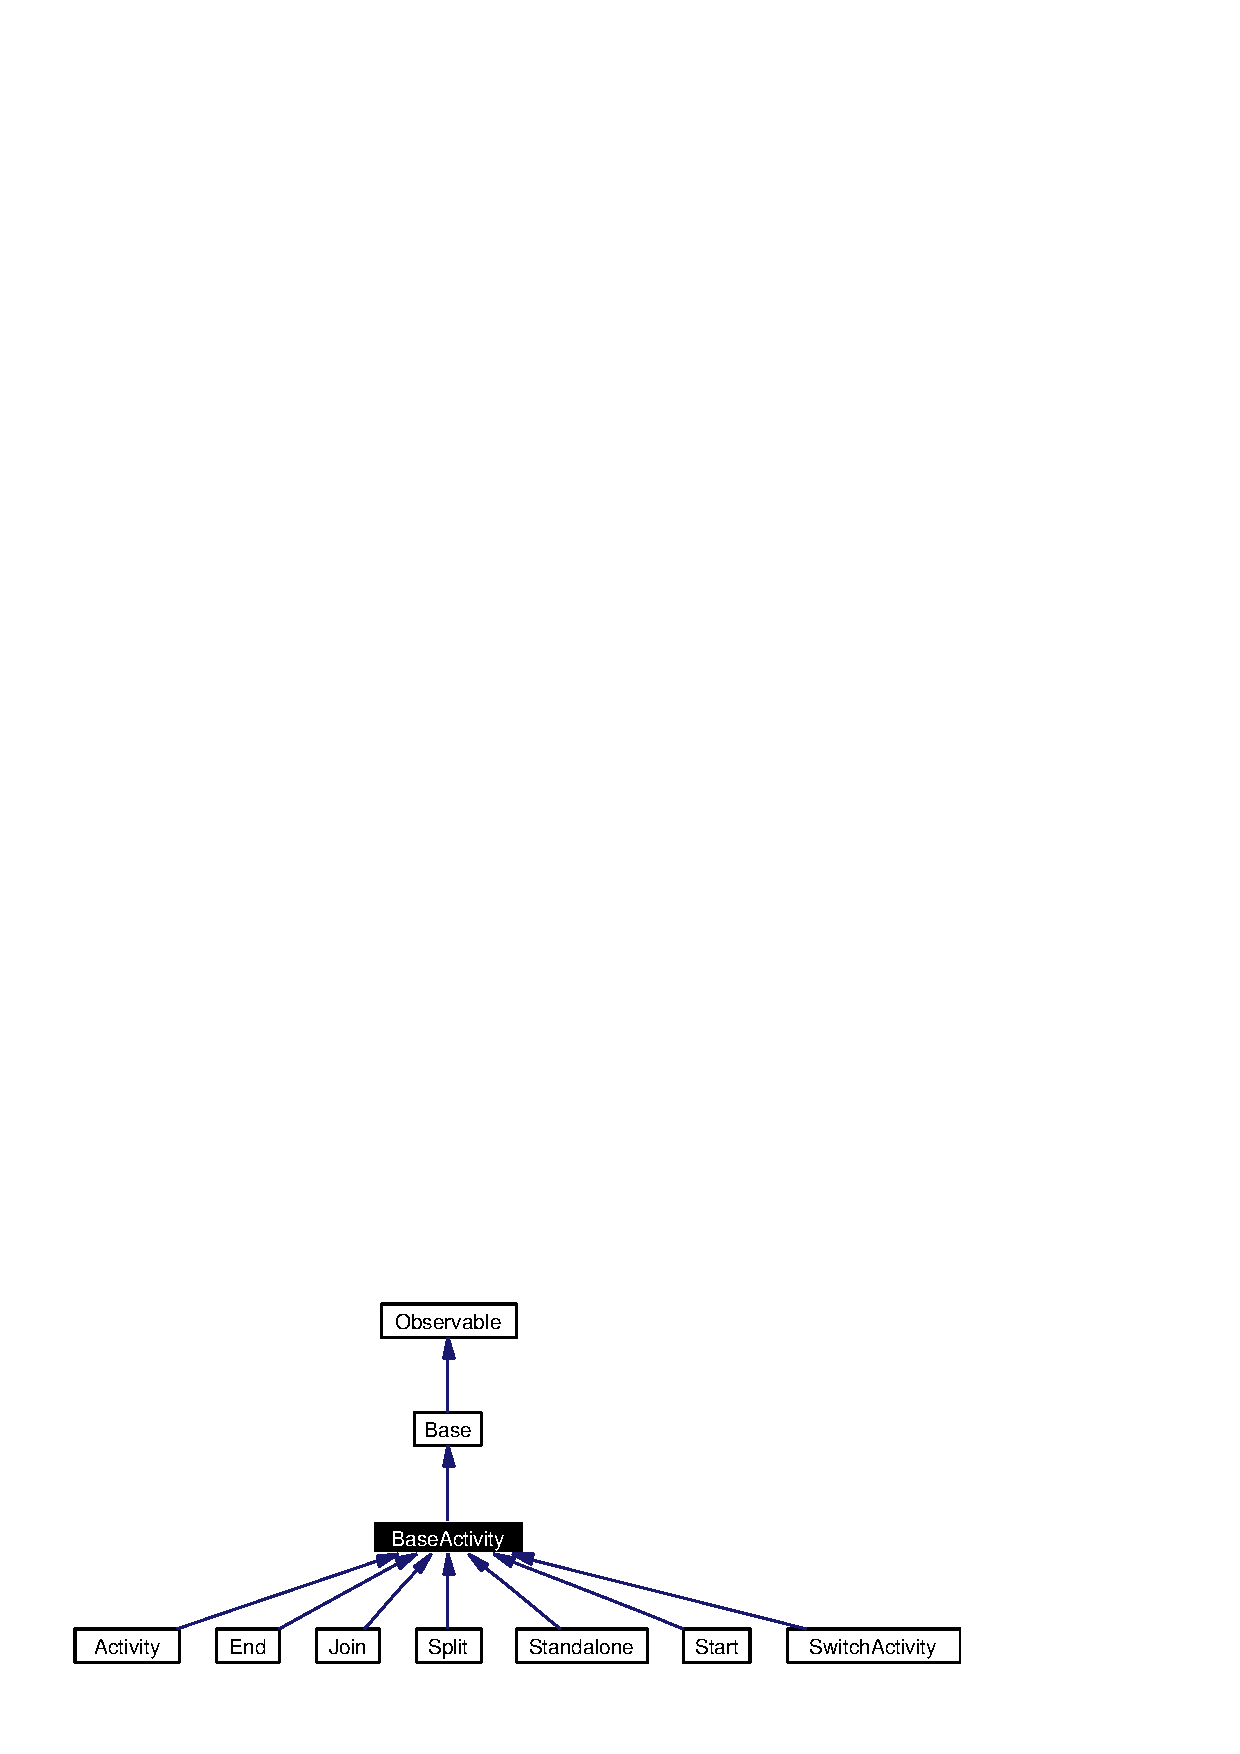
\includegraphics[width=230pt]{classBaseActivity__inherit__graph}
\end{center}
\end{figure}
Collaboration diagram for Base\-Activity:\begin{figure}[H]
\begin{center}
\leavevmode
\includegraphics[width=54pt]{classBaseActivity__coll__graph}
\end{center}
\end{figure}
\subsection*{Public Member Functions}
\begin{CompactItemize}
\item 
{\bf set\-Db} (\$db)\label{classBaseActivity_a0}

\item 
{\bf Base\-Activity} (\$db)\label{classBaseActivity_a1}

\item 
{\bf get\-Activity} (\$activity\-Id)
\item 
{\bf get\-User\-Roles} (\$user)
\item 
{\bf get\-Activity\-Role\-Names} ()
\item 
{\bf get\-Normalized\-Name} ()
\item 
{\bf set\-Normalized\-Name} (\$name)
\item 
{\bf set\-Name} (\$name)
\item 
{\bf get\-Name} ()
\item 
{\bf set\-Description} (\$desc)
\item 
{\bf get\-Description} ()
\item 
{\bf set\-Is\-Interactive} (\$is)
\item 
{\bf is\-Interactive} ()
\item 
{\bf set\-Is\-Auto\-Routed} (\$is)
\item 
{\bf is\-Auto\-Routed} ()
\item 
{\bf set\-Process\-Id} (\$pid)
\item 
{\bf get\-Process\-Id} ()
\item 
{\bf get\-Activity\-Id} ()
\item 
{\bf set\-Activity\-Id} (\$id)
\item 
{\bf get\-Roles} ()
\item 
{\bf set\-Roles} (\$roles)
\end{CompactItemize}
\subsection*{Public Attributes}
\begin{CompactItemize}
\item 
{\bf \$name}\label{classBaseActivity_o0}

\item 
{\bf \$normalized\-Name}\label{classBaseActivity_o1}

\item 
{\bf \$description}\label{classBaseActivity_o2}

\item 
{\bf \$is\-Interactive}\label{classBaseActivity_o3}

\item 
{\bf \$is\-Auto\-Routed}\label{classBaseActivity_o4}

\item 
{\bf \$roles} = Array()\label{classBaseActivity_o5}

\item 
{\bf \$outbound} = Array()\label{classBaseActivity_o6}

\item 
{\bf \$inbound} = Array()\label{classBaseActivity_o7}

\item 
{\bf \$p\-Id}\label{classBaseActivity_o8}

\item 
{\bf \$activity\-Id}\label{classBaseActivity_o9}

\end{CompactItemize}


\subsection{Detailed Description}
This class represents activities, and must be derived for each activity type supported in the system. Derived activities extending this class can be found in the activities subfolder. This class is observable. 



Definition at line 11 of file Base\-Activity.php.

\subsection{Member Function Documentation}
\index{BaseActivity@{Base\-Activity}!getActivity@{getActivity}}
\index{getActivity@{getActivity}!BaseActivity@{Base\-Activity}}
\subsubsection{\setlength{\rightskip}{0pt plus 5cm}Base\-Activity::get\-Activity (\$ {\em activity\-Id})}\label{classBaseActivity_a2}


Factory method returning an activity of the desired type loading the information from the database. 

Definition at line 38 of file Base\-Activity.php.

References is\-Auto\-Routed(), and is\-Interactive().\index{BaseActivity@{Base\-Activity}!getActivityId@{getActivityId}}
\index{getActivityId@{getActivityId}!BaseActivity@{Base\-Activity}}
\subsubsection{\setlength{\rightskip}{0pt plus 5cm}Base\-Activity::get\-Activity\-Id ()}\label{classBaseActivity_a17}


Gets the activity\-Id 

Definition at line 177 of file Base\-Activity.php.\index{BaseActivity@{Base\-Activity}!getActivityRoleNames@{getActivityRoleNames}}
\index{getActivityRoleNames@{getActivityRoleNames}!BaseActivity@{Base\-Activity}}
\subsubsection{\setlength{\rightskip}{0pt plus 5cm}Base\-Activity::get\-Activity\-Role\-Names ()}\label{classBaseActivity_a4}


Returns an Array of asociative arrays with role\-Id and name for the given user 

Definition at line 105 of file Base\-Activity.php.\index{BaseActivity@{Base\-Activity}!getDescription@{getDescription}}
\index{getDescription@{getDescription}!BaseActivity@{Base\-Activity}}
\subsubsection{\setlength{\rightskip}{0pt plus 5cm}Base\-Activity::get\-Description ()}\label{classBaseActivity_a10}


Gets the activity description 

Definition at line 142 of file Base\-Activity.php.\index{BaseActivity@{Base\-Activity}!getName@{getName}}
\index{getName@{getName}!BaseActivity@{Base\-Activity}}
\subsubsection{\setlength{\rightskip}{0pt plus 5cm}Base\-Activity::get\-Name ()}\label{classBaseActivity_a8}


Gets the activity name 

Definition at line 132 of file Base\-Activity.php.\index{BaseActivity@{Base\-Activity}!getNormalizedName@{getNormalizedName}}
\index{getNormalizedName@{getNormalizedName}!BaseActivity@{Base\-Activity}}
\subsubsection{\setlength{\rightskip}{0pt plus 5cm}Base\-Activity::get\-Normalized\-Name ()}\label{classBaseActivity_a5}


Returns the normalized name for the activity 

Definition at line 117 of file Base\-Activity.php.\index{BaseActivity@{Base\-Activity}!getProcessId@{getProcessId}}
\index{getProcessId@{getProcessId}!BaseActivity@{Base\-Activity}}
\subsubsection{\setlength{\rightskip}{0pt plus 5cm}Base\-Activity::get\-Process\-Id ()}\label{classBaseActivity_a16}


Gets the process\-Id for this activity 

Definition at line 172 of file Base\-Activity.php.\index{BaseActivity@{Base\-Activity}!getRoles@{getRoles}}
\index{getRoles@{getRoles}!BaseActivity@{Base\-Activity}}
\subsubsection{\setlength{\rightskip}{0pt plus 5cm}Base\-Activity::get\-Roles ()}\label{classBaseActivity_a19}


Gets array with role\-Ids asociated to this activity 

Definition at line 187 of file Base\-Activity.php.\index{BaseActivity@{Base\-Activity}!getUserRoles@{getUserRoles}}
\index{getUserRoles@{getUserRoles}!BaseActivity@{Base\-Activity}}
\subsubsection{\setlength{\rightskip}{0pt plus 5cm}Base\-Activity::get\-User\-Roles (\$ {\em user})}\label{classBaseActivity_a3}


Returns an Array of role\-Ids for the given user 

Definition at line 93 of file Base\-Activity.php.\index{BaseActivity@{Base\-Activity}!isAutoRouted@{isAutoRouted}}
\index{isAutoRouted@{isAutoRouted}!BaseActivity@{Base\-Activity}}
\subsubsection{\setlength{\rightskip}{0pt plus 5cm}Base\-Activity::is\-Auto\-Routed ()}\label{classBaseActivity_a14}


Gets if the activity is auto routed 

Definition at line 162 of file Base\-Activity.php.

Referenced by get\-Activity().\index{BaseActivity@{Base\-Activity}!isInteractive@{isInteractive}}
\index{isInteractive@{isInteractive}!BaseActivity@{Base\-Activity}}
\subsubsection{\setlength{\rightskip}{0pt plus 5cm}Base\-Activity::is\-Interactive ()}\label{classBaseActivity_a12}


Returns if the activity is interactive 

Definition at line 152 of file Base\-Activity.php.

Referenced by get\-Activity().\index{BaseActivity@{Base\-Activity}!setActivityId@{setActivityId}}
\index{setActivityId@{setActivityId}!BaseActivity@{Base\-Activity}}
\subsubsection{\setlength{\rightskip}{0pt plus 5cm}Base\-Activity::set\-Activity\-Id (\$ {\em id})}\label{classBaseActivity_a18}


Sets the activity\-Id 

Definition at line 182 of file Base\-Activity.php.\index{BaseActivity@{Base\-Activity}!setDescription@{setDescription}}
\index{setDescription@{setDescription}!BaseActivity@{Base\-Activity}}
\subsubsection{\setlength{\rightskip}{0pt plus 5cm}Base\-Activity::set\-Description (\$ {\em desc})}\label{classBaseActivity_a9}


Sets the activity description 

Definition at line 137 of file Base\-Activity.php.\index{BaseActivity@{Base\-Activity}!setIsAutoRouted@{setIsAutoRouted}}
\index{setIsAutoRouted@{setIsAutoRouted}!BaseActivity@{Base\-Activity}}
\subsubsection{\setlength{\rightskip}{0pt plus 5cm}Base\-Activity::set\-Is\-Auto\-Routed (\$ {\em is})}\label{classBaseActivity_a13}


Sets if the activity is auto-routed 

Definition at line 157 of file Base\-Activity.php.\index{BaseActivity@{Base\-Activity}!setIsInteractive@{setIsInteractive}}
\index{setIsInteractive@{setIsInteractive}!BaseActivity@{Base\-Activity}}
\subsubsection{\setlength{\rightskip}{0pt plus 5cm}Base\-Activity::set\-Is\-Interactive (\$ {\em is})}\label{classBaseActivity_a11}


Sets if the activity is interactive 

Definition at line 147 of file Base\-Activity.php.\index{BaseActivity@{Base\-Activity}!setName@{setName}}
\index{setName@{setName}!BaseActivity@{Base\-Activity}}
\subsubsection{\setlength{\rightskip}{0pt plus 5cm}Base\-Activity::set\-Name (\$ {\em name})}\label{classBaseActivity_a7}


Sets the name for the activity 

Definition at line 127 of file Base\-Activity.php.\index{BaseActivity@{Base\-Activity}!setNormalizedName@{setNormalizedName}}
\index{setNormalizedName@{setNormalizedName}!BaseActivity@{Base\-Activity}}
\subsubsection{\setlength{\rightskip}{0pt plus 5cm}Base\-Activity::set\-Normalized\-Name (\$ {\em name})}\label{classBaseActivity_a6}


Sets normalized name for the activity 

Definition at line 122 of file Base\-Activity.php.\index{BaseActivity@{Base\-Activity}!setProcessId@{setProcessId}}
\index{setProcessId@{setProcessId}!BaseActivity@{Base\-Activity}}
\subsubsection{\setlength{\rightskip}{0pt plus 5cm}Base\-Activity::set\-Process\-Id (\$ {\em pid})}\label{classBaseActivity_a15}


Sets the process\-Id for this activity 

Definition at line 167 of file Base\-Activity.php.\index{BaseActivity@{Base\-Activity}!setRoles@{setRoles}}
\index{setRoles@{setRoles}!BaseActivity@{Base\-Activity}}
\subsubsection{\setlength{\rightskip}{0pt plus 5cm}Base\-Activity::set\-Roles (\$ {\em roles})}\label{classBaseActivity_a20}


Sets roles for this activities, shoule receive an array of role\-Ids 

Definition at line 193 of file Base\-Activity.php.

The documentation for this class was generated from the following file:\begin{CompactItemize}
\item 
Base\-Activity.php\end{CompactItemize}
